\documentclass[a4paper,fontset=fandol]{ctexart}

\usepackage{amsmath,amssymb,amsthm,physics,fancyhdr,geometry,hyperref,graphicx,enumitem,upgreek,booktabs,multirow}

\geometry{vmargin=2cm,hmargin=2.5cm}

\pagestyle{fancy}
\fancyhf{}
\fancyfoot[C]{\thepage}
\renewcommand{\headrulewidth}{0pt}

\usepackage{titlesec}
\titleformat{\section}
{\normalfont\Large\bfseries}{天文馆比赛\thesection:}{0.5em}{}

\newcommand{\points}[1]{\par % 确保换行
	\noindent % 取消缩进
	\hfill (#1分)% 右对齐并添加分数
	\vspace{1em}
	}

%\parskip=0.5em

\hypersetup{colorlinks}

\begin{document}
	{
		\Large\bfseries\noindent 天文馆比赛:\hspace{0.5em}流程
	}
	
	你有30分钟的时间来阅读问题和准备, 在天文馆内有30分钟, 以及30分钟来处理你的观测结果并完成答题纸. 
	
	准备区位于天文馆外. 前往与你的团队名称匹配的, 用于团体赛的桌子. 它也会标有分配给你的扇区、排和座位号, 这些与你在天文馆内的安排相同. 
	
	仅当监考员发出``开始''命令时才打开信封. 你有30分钟, 监考员会告知剩余时间, 例如``还剩10分钟'', ``还剩2分钟''. 在``停止''命令发出时, 停止工作, 但在看到``现在开始''的信号前不要离开你的座位. 只带走你的试题纸、写字板和笔/铅笔 (留下星图) . 按照指示进入天文馆, 与其他参与者保持距离, 并找到你的位置. 不要与其他参与者交谈. 
	
	在比赛期间, 你可以站起来以获得更好的视野, 但不要四处走动、更换座位、与其他参与者交谈, 或将你的光源照射他人或天空. \textbf{光源必须始终指向下方}. 
	
	这一轮分为3个10分钟的部分. 第一部分用于问题1. 第二部分用于问题2. 第三部分用于问题3. 在结束前5分钟、2分钟和1分钟, 天空将短暂显示警告. 
	
	在比赛结束时, 在座位上等待, 直到看到``现在开始''的信号. 按照指示前往处理区, 并像之前一样找到与你的团队匹配的桌子 (留下光源) . 与其他参与者保持距离, 不要与他们交谈. 等所有人都坐下后, 你将有30分钟的时间来处理你的观测结果并完成答题纸 (将提供计算器、几何工具等, 以及显示剩余时间的时钟). 在30分钟结束时, 将你的答题纸放入信封, 并在桌子上等待, 直到被告知离开该区域. 
	
	\newpage
	\section{星空知识}
	
	投影仪将展示从赤道附近 (0$^\circ$N, 19$^\circ$E) 看到的星空. 星空的旋转将在(a)部分时暂停约2分钟, 然后它将开始旋转以进行(b)和(c)部分. (b)和(c)部分的对象将同时显示. 
	
	{\hfill (投影时间 10分钟)}
	
	\begin{enumerate}[label=(\alph*)]
		\item 将展示一场流星雨. 确定辐射点所在的星座, 并估计其赤经和赤纬坐标. 
		
		\begin{table}[!h]
			\centering
			\begin{tabular}{|c|l|l|}
				\hline
				星座~~~~~~~~~~ & 赤经~~~~~~~~~~ & 赤纬~~~~~~~~~~ \\
				\hline
				&&\\
				\hline
			\end{tabular}
		\end{table}
		\points{3}
		
		\vspace{0em}
		\item 识别下列在天空中可见的变星处于亮度较低 (写`DIM') 或较高 (写`BRIGHT') 的状态. 星表中的星等和每颗星的星等范围都已给出. 
		
		\begin{table}[!h]
			\centering
			\begin{tabular}{|l|c|c|c|}
				\hline
				名称 & 星表星等 & 星等范围 & DIM / BRIGHT \\
				\hline
				$\gamma$ Cas (\textit{Cih}) & 2 & 1.6---3.0 & \\
				\hline
				$\delta$ Cep & 4 & 3.5---4.4 & \\
				\hline
				$\mu$ Cep (\textit{Erakis}) & 4 & 3.4---5.1 & \\
				\hline
				$\beta$ Per (\textit{Algol}) & 2 & 2.2---3.4 & \\
				\hline
				\textit{o} Cet (\textit{Mira}) & 3.5 & 2.0---10.1 & \\
				\hline
				$\chi$ Cyg & 4.5 & 3.3---14.1 & \\
				\hline
				L$^2$ Pup & 4.5 & 2.6---6 & \\
				\hline
				$\delta$ Sco (\textit{Dschubba}) & 2 & 1.6---2.3 & \\
				\hline
			\end{tabular}
		\end{table}
		\points{8}
		
		\vspace{0em}
		\item 识别标有边界的星座并给出它们的IAU缩写. 
		\points{9}
	\end{enumerate}
	\points{总计:20}
	
	\newpage
	\section{逆行火星}
	
	投影仪将展示火星相对于背景恒星在一个可见季节 (1.5年) 内的移动, 从日出开始, 选择这个时间点是因为火星在冲时将处于最大黄纬. 
	
	黄道也会被展示出来, 标有一年中太阳的位置和当前日期. 太阳始终在地平线以下. 
	
	火星的会合周期 = 780天. 
	
	{\hfill (投影时间: 10分钟)}
	
	\begin{enumerate}[label=(\alph*)]
		\item 记录以下量:
		\begin{table}[!h]
			\centering
			\begin{tabular}{|l|c|}
				\hline
				\multirow{2}{*}{i.\,\,\,\,四分位的日期 (当火星的黄经差为90$^\circ$时) }&~~~~~~~~~~~~~~~~~~~~~~~~~~~~~~~~~~~\\
				\cline{2-2}
				&\\
				\hline
				\multirow{2}{*}{ii.\,\,\,\parbox[t]{30em}{逆行运动开始的日期和逆行运动结束的日期}}&\\
				\cline{2-2}
				&\\
				\hline
				iii.\,\,冲的日期&\\
				\hline
				iv.\,\,冲位置的黄纬&\\
				\hline
				v.\,\,\,\,行星所形成的环在黄经上的宽度&\\
				\hline
			\end{tabular}
		\end{table}
		\points{8}
	\end{enumerate}
	
	根据你的观测, 并假设地球和火星的轨道是圆形的, 
	
	\begin{enumerate}[label=(\alph*),start=2]
		\item 在答题纸上, 标记太阳、地球和火星在冲和四分位时刻在地心系统中的位置, 并确定火星的轨道半径, 以天文单位为单位, 用纯几何方法 (不使用开普勒定律). 在答题纸上展示你的方法. 
		\points{9}
		
		\vspace{0em}
		\item 推导出火星轨道对黄道的倾角. \hfill(3点)
	\end{enumerate}
	\points{总计:20}
	
	\newpage
	
	{\Large\bfseries 答题纸}
	
	\begin{figure}[!h]
		\centering
		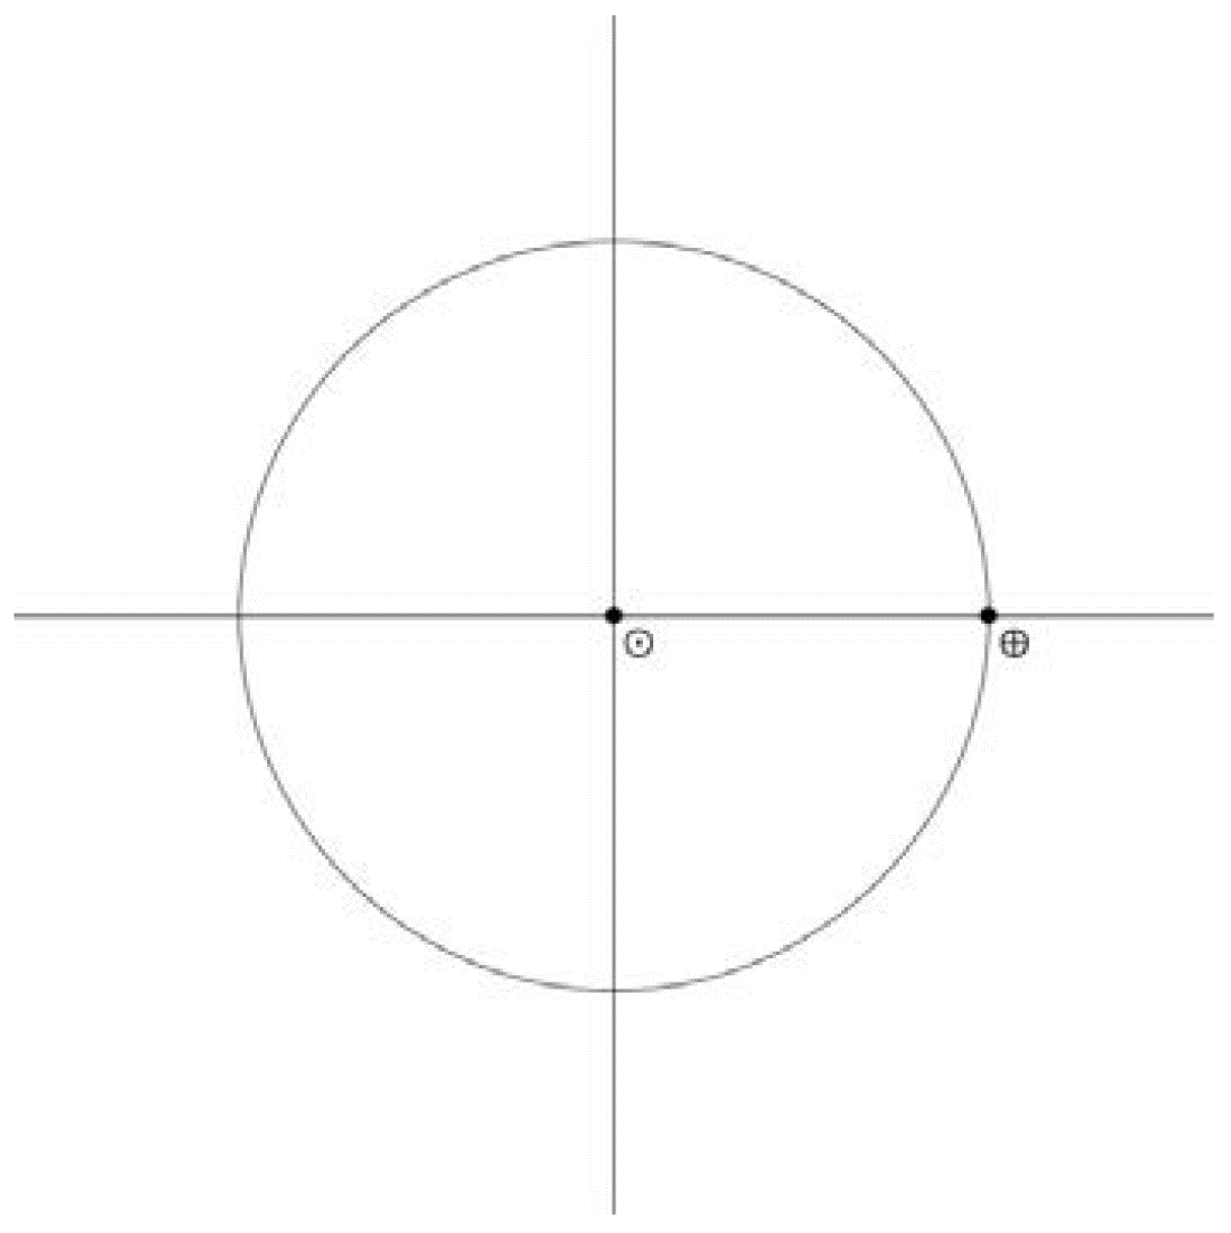
\includegraphics{fig/1.png}
	\end{figure}
	
	\newpage
	\section{TRAPPIST-1}
	
	外星人发现地球的天文学家通过观察众多的凌星现象发现了TRAPPIST-1系统中的行星. 他们用他们的飞碟 (类似于你在观测比赛中的那一个) 带你去了TRAPPIST-1的第五颗行星 (指定为 $f$) , 并要求你向他们展示地球人用来揭开系统参数的方法. 将展示一个以地球小时显示时间的时钟. 整个演示将持续520小时 (1秒代表1小时) . 
	
	{\hfill (投影时间 10分钟)}
	
	基于你的观测 (你可以使用最后一页做观测笔记) , 
	
	\begin{enumerate}[label=(\alph*)]
		\item 确定你所在行星的以下量 (使用地球小时表示时间) :\hfill(7分)
		
		\begin{tabular}{|l|l|}
			\hline
			i.\,\,\,\,\,恒星日长 [h]&~~~~~~~~~~~~~~~~~~~~~~~~~~~~~~~~~~~\\
			\hline
			ii.\,\,\,\,轨道周期 [h]&\\
			\hline
			iii.\,\,\,``太阳''日长 [h]&\\
			\hline
			iv.\,\,\,圆形轨道&YES / NO\\
			\hline
			v.\,\,\,\,黄赤交角 (轴倾角) &\\
			\hline
		\end{tabular}
		
		\item 以及每颗行星 $b$、$c$、$d$ 和 $e$ 的以下量:\hfill(16分)
		
		\begin{tabular}{|l|l|l|l|l|}
			\hline
			&$b$&$c$&$d$&$e$\\
			\hline
			合日周期 [h]&~~~~~~~~~~~~~~~~~~~~&~~~~~~~~~~~~~~~~~~~~&~~~~~~~~~~~~~~~~~~~~&~~~~~~~~~~~~~~~~~~~~\\
			\hline
			最大黄经差 [$^\circ$]&&&&\\
			\hline
		\end{tabular}
		
		\item 计算每颗行星的轨道周期 (以小时为单位) 以及半长轴 (以tau为单位, 其中1 tau = ``TRAPPIST-1$f$天文单位'' = TRAPPIST-1$f$轨道的半长轴):
		
		\hfill(8分)
		
		\begin{tabular}{|l|l|l|l|l|}
			\hline
			&$b$&$c$&$d$&$e$\\
			\hline
			轨道周期 [h]&~~~~~~~~~~~~~~~~~~~~&~~~~~~~~~~~~~~~~~~~~&~~~~~~~~~~~~~~~~~~~~&~~~~~~~~~~~~~~~~~~~~\\
			\hline
			半长轴 [tau]&&&&\\
			\hline
		\end{tabular}
		
		\item ‘引力共振’一词用来描述系统中两颗行星的轨道周期比接近两个整数比的现象. 下面的表格列出了在TRAPPIST-1系统中观察到的一些共振. 如果有出现, 找出哪对行星对应于列出的每种共振. \points{4}
		
		\vspace{0em}
		\begin{center}
			\begin{tabular}{|l|l|}
				\hline
				共振~~~~~~~~~~&行星对~~~~~~~\\
				\hline
				3:2&\\
				\hline
				8:5&\\
				\hline
				5:3&\\
				\hline
				8:3&\\
				\hline
				4:1&\\
				\hline
				6:1&\\
				\hline
			\end{tabular}
		\end{center}
		\end{enumerate}
		\points{总计:35}
	
\end{document}